% Area Personale
L’utente registrato e che ha effettuato l’accesso nella piattaforma web, avrà un’area personale nella quale:

\begin{itemize}
\item Visualizzare i propri dati personali (\S{7.1}),
\item Modificare la password di accesso al sistema (\S{7.2}),
\item Suggerire un profilo Instagram che potrebbe essere utile alla piattaforma (\S{7.3}),
\item Visualizzare e gestire la propria lista dei preferiti (\S{7.4}).
\end{itemize}

È possibile scegliere una di queste operazioni dalla sezione “Area Personale” (sia per la versione desktop che mobile), la quale aprirà una nuova finestra a seconda della funzionalità scelta.

\subsection{Visualizza dati personali}

L’utente registrato e che ha effettuato l’accesso alla piattaforma web può visualizzare i propri dati personali inseriti in fase di registrazione.

I dati personali che un utente può visualizzare nella sua Area Personale (alla sezione “Dati Personali”) sono:

\begin{itemize}
\item Nome,
\item Cognome,
\item Indirizzo e-mail.
\end{itemize}

\begin{figure}[H]
\centering
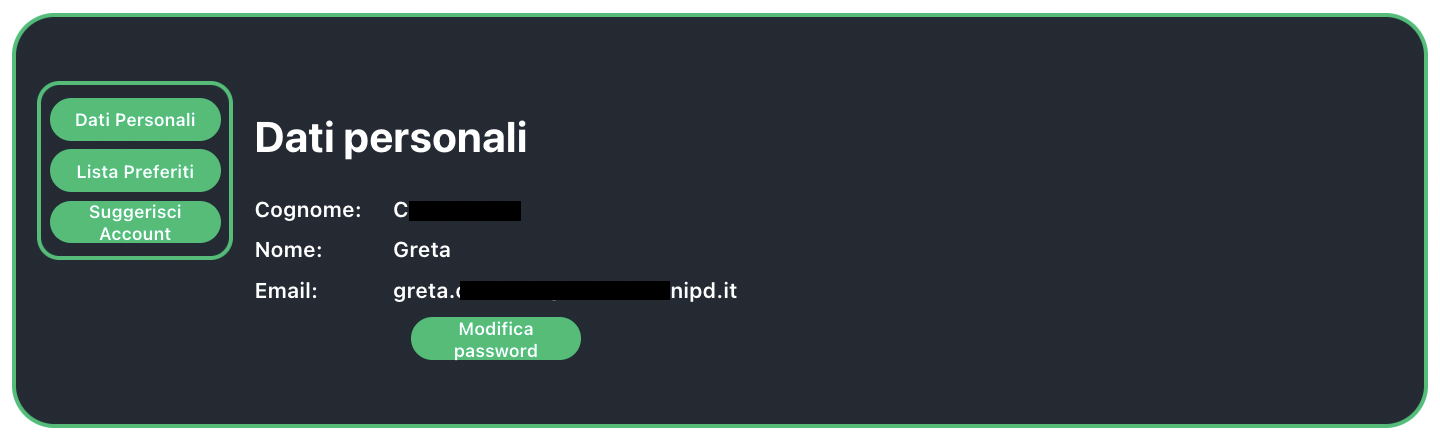
\includegraphics[scale=0.4]{./images/AreaPersonale/DatiPersonali.png} 
\caption{Suggerisci profilo}
\end{figure}

Da questa schermata l’utente può anche modificare la propria password (come indicato nel paragrafo che segue).

\subsection{Modifica password}

L’utente registrato e che ha effettuato il proprio accesso al sistema ha la possibilità di modificare la propria password di accesso.

Per fare ciò, dalla sezione denominata “Dati Personali”, l'utente dovrà cliccare sul bottone “\textbf{Modifica Password}” ed inserire una nuova password, avendo cura di inserire almeno: 8 caratteri e che contengono almeno una lettera maiuscola, una minuscola, un numero ed un simbolo tra i seguenti: @ \$ ! \% * ? \&{}.

\begin{figure}[H]
\centering
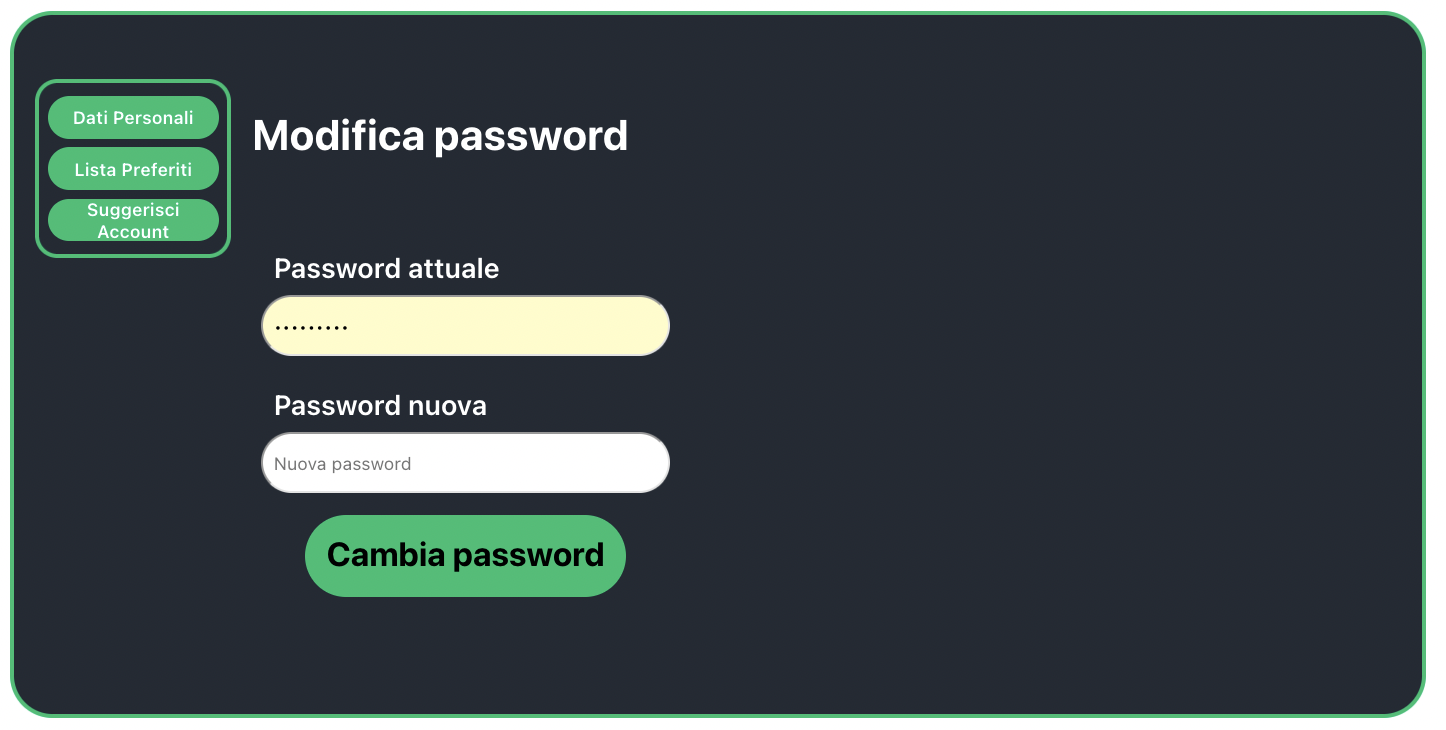
\includegraphics[scale=0.4]{./images/AreaPersonale/CambiaPassword.png} 
\caption{Suggerisci profilo}
\end{figure}

\subsection{Suggerisci un profilo}

Un utente registrato alla piattaforma e che ha effettuato l’accesso ha l’opportunità di suggerire un profilo Instagram al sistema.

Per fare ciò, dalla pagina “Area Personale” un utente può cliccare sulla voce “Suggerisci un profilo”, dalla quale comparirà una casella di testo:

\begin{figure}[H]
\centering
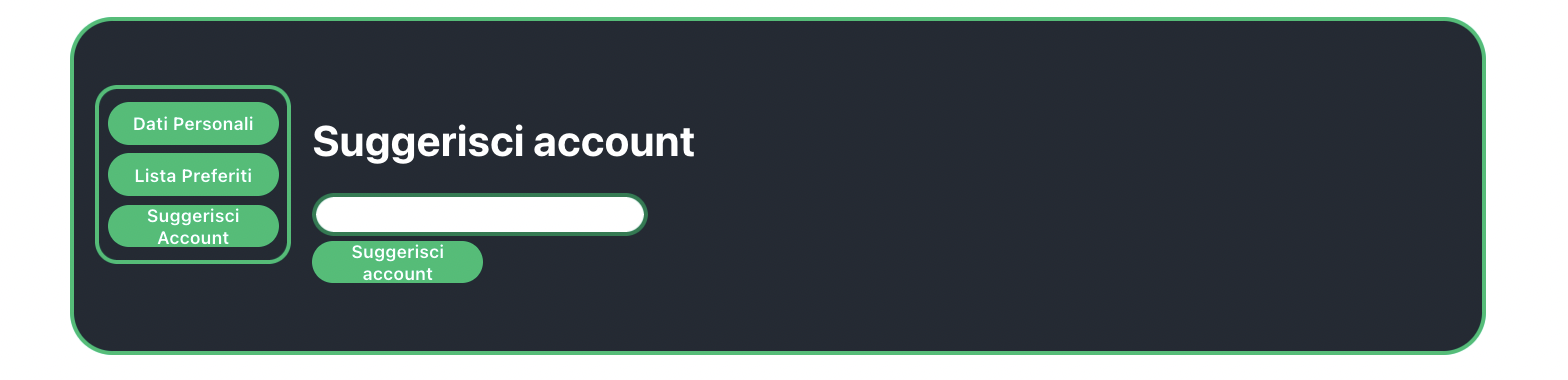
\includegraphics[scale=0.4]{./images/AreaPersonale/SuggerisciAccount.png} 
\caption{Suggerisci profilo}
\end{figure}

Al suo interno, l’utente potrà inserire il nome utente del profilo Instagram da suggerire alla piattaforma. 

Una volta suggerito il profilo, si potranno ottenere quattro diverse risposte:

\begin{itemize}
\item Profilo aggiunto correttamente,
\item Profilo già presente a sistema,
\item Profilo inesistente,
\item Profilo privato.
\end{itemize}

Nel caso in cui il profilo suggerito venga aggiunto a sistema correttamente:

\begin{figure}[H]
\centering
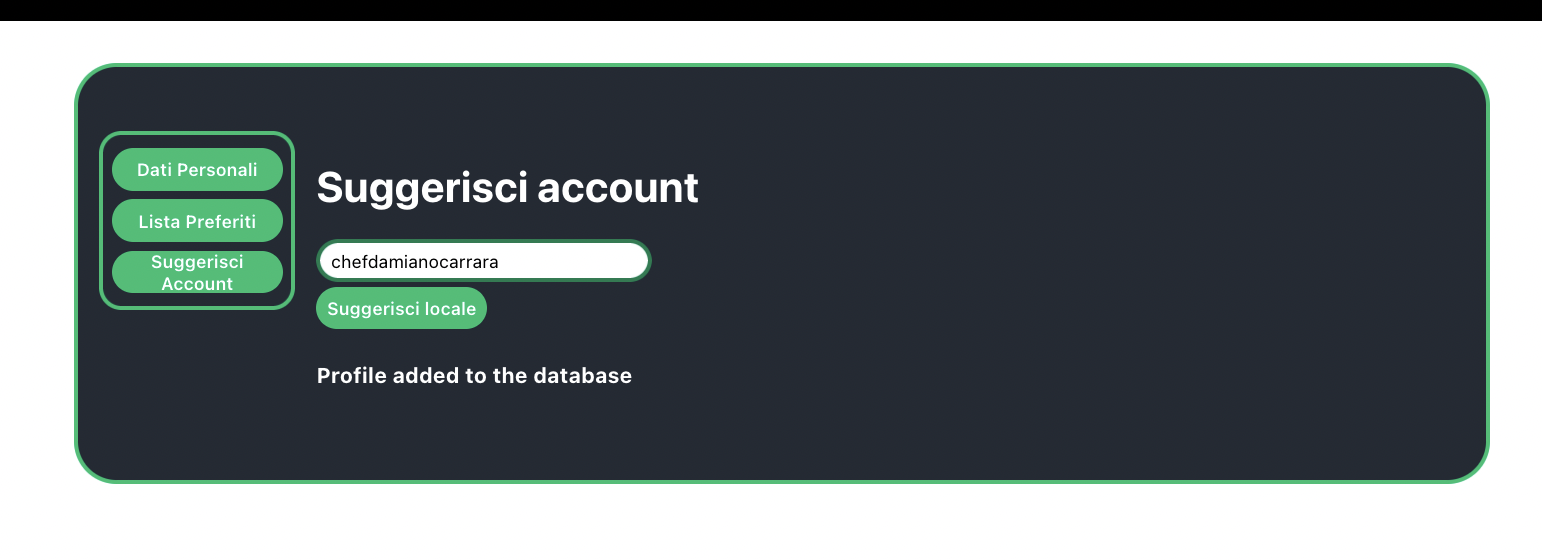
\includegraphics[scale=0.4]{./images/AreaPersonale/ProfiloAggiunto.png} 
\caption{Profilo suggerito aggiunto correttamente}
\end{figure}

Nel caso in cui il profilo sia già presente a sistema:

\begin{figure}[H]
\centering
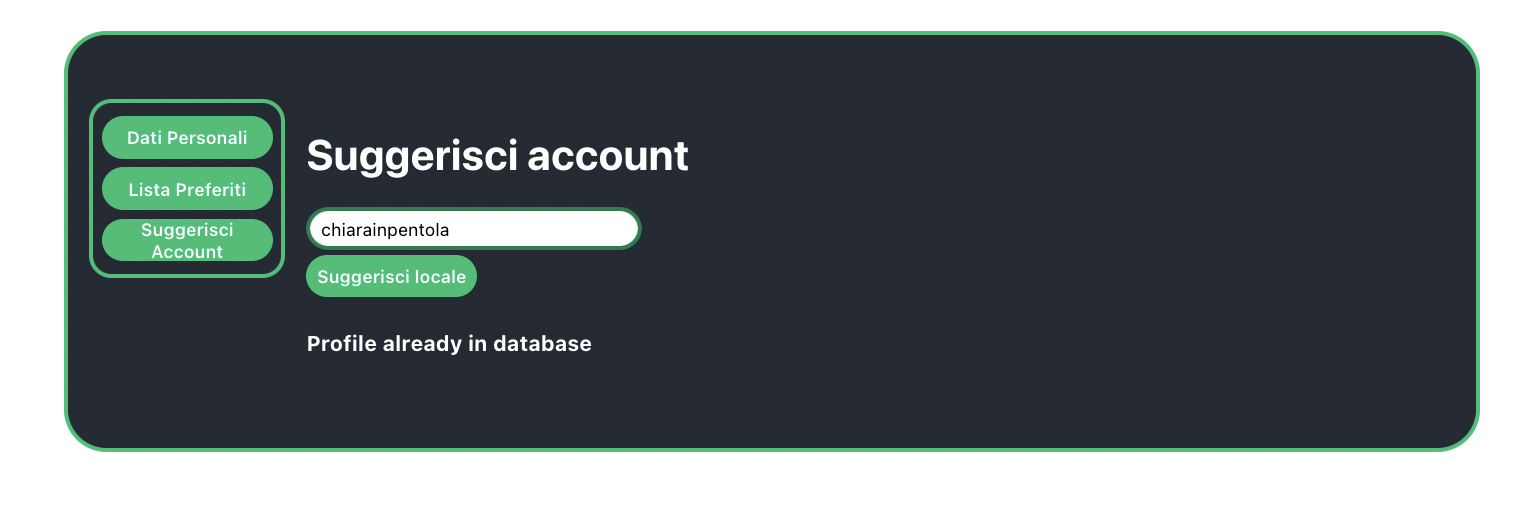
\includegraphics[scale=0.4]{./images/AreaPersonale/ProfiloPresenteNelDB.png} 
\caption{Profilo suggerito già presente a sistema}
\end{figure}

Nel caso in cui il profilo suggerito non esiste su Instagram:

\begin{figure}[H]
\centering
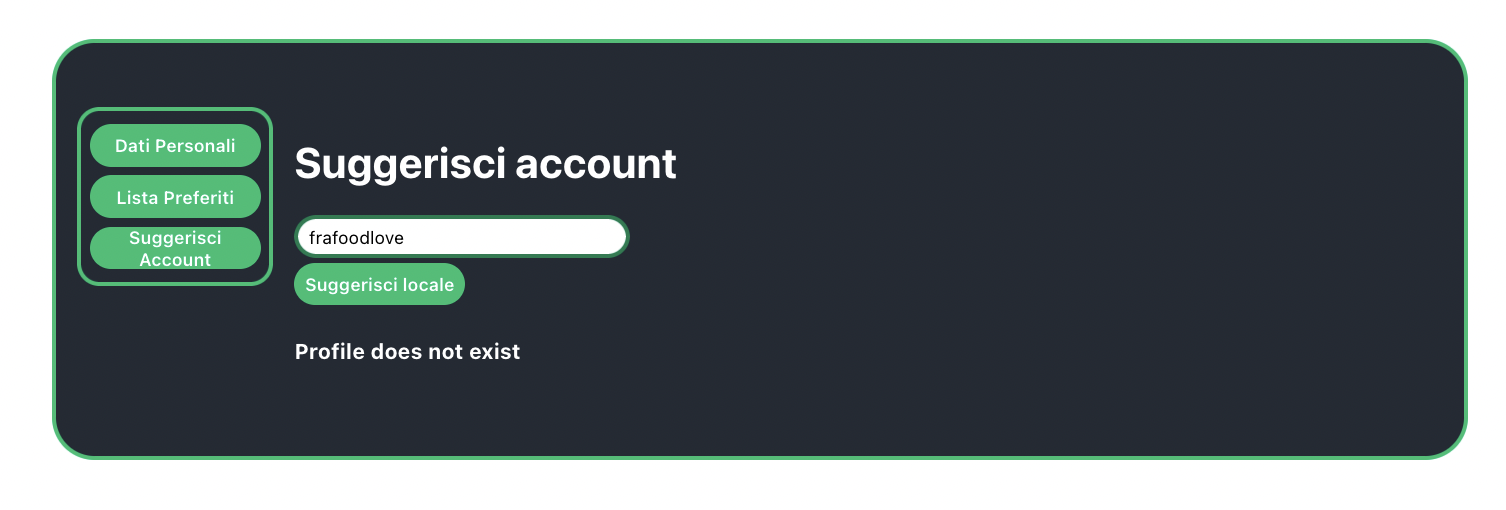
\includegraphics[scale=0.4]{./images/AreaPersonale/ProfiloInesistente.png} 
\caption{Profilo suggerito inesistente}
\end{figure}

Infine, è possibile che un profilo suggerito sia privato:

\begin{figure}[H]
\centering
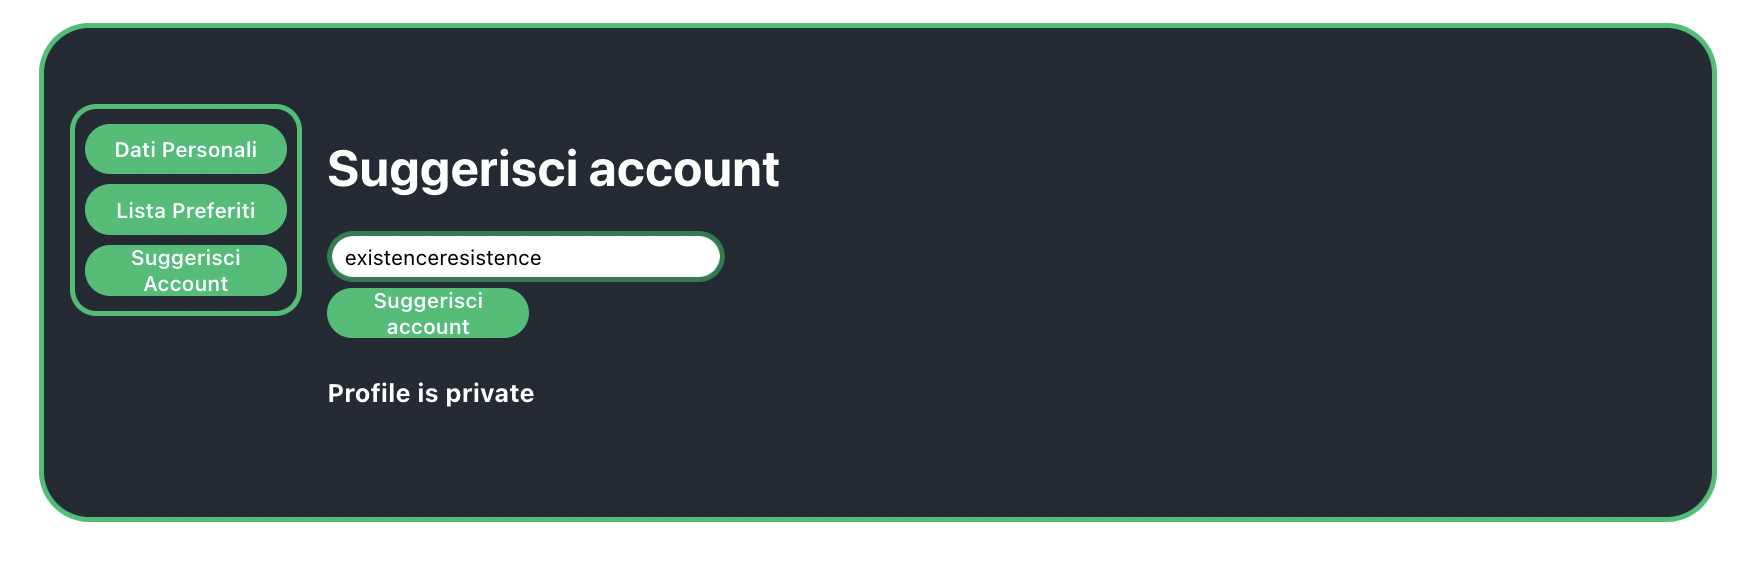
\includegraphics[scale=0.4]{./images/AreaPersonale/ProfiloPrivato.png} 
\caption{Profilo suggerito aggiunto correttamente}
\end{figure}

\subsection{Lista dei preferiti}

Un utente registrato e che ha effettuato l’accesso alla piattaforma ha l’opportunità rimuovere locali dalla propria lista dei preferiti direttamente dall'Area Personale. \\

Dalla sezione “Area Personale”, l’utente autenticato può cliccare su “Lista dei preferiti” dove visualizzerà o una lista vuota, nel caso nella lista non ci sia alcun locale preferito, o una lista con dei locali presenti a sistema.

\begin{figure}[H]
\centering
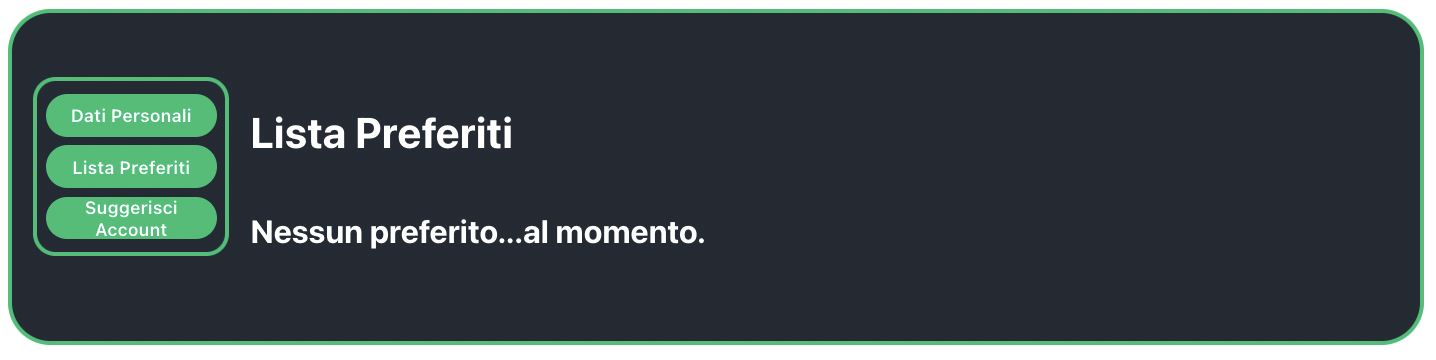
\includegraphics[scale=0.4]{./images/AreaPersonale/ListaPreferiti.png} 
\caption{Lista dei locali preferiti}
\end{figure}

L’utente può rimuovere un locale dalla lista dei preferiti semplicemente cliccando sull’icona del cestino.

In questo modo, il locale verrà rimosso dalla lista e sarà necessario cercarlo (tramite la ricerca \S{8.1}) per aggiungerlo nuovamente. Questo meccanismo di aggiungere e rimuovere un locale dalla lista dei preferiti è una funzionalità che non è ancora stata implementata.
